\chapter*{2 Versuchsdurchführung und Auswertung}
\addcontentsline{toc}{chapter}{2 Versuchsdurchführung und Auswertung}
\setcounter{chapter}{2}
\setcounter{section}{0}
\setcounter{subsection}{0}
 
    \section{Versuch 1 - Oberflächenspannung von Wasser und Ethanol mit der Abreißmethode}
    \label{sec:Versuch1}
        
        \subsection{Aufbau}

            \begin{figure}[H]
                \centering
                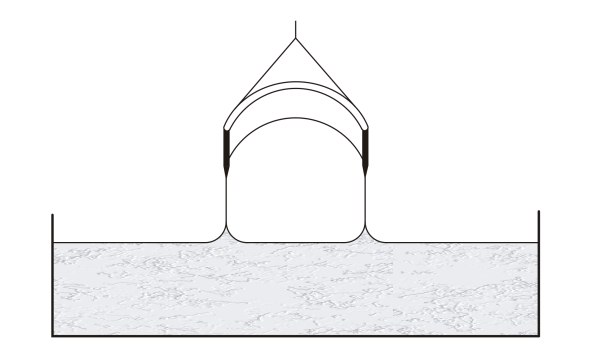
\includegraphics[width=0.8\textwidth]{bilder/Versuch1_Aufbau.png}
                \caption{Versuchsaufbau Versuch 1 \ref{an:Anleitung}}
                \label{fig:Versuch1_Aufbau}
            \end{figure}

            Um die Oberflächenspannung einer Flüssigkeit mit der Abreißmethode zu bestimmen,
            braucht man einen Metallring, einen Federkraftmesser und eine mit einer Flüssigkeit gefüllten Schale. Nun taucht man den Ring in die Flüssigkeit und misst die maximale Kraft $\mathrm{F}$, die nötig ist um den Ring wieder herauszuziehen. Die Oberflächenspannung $\sigma$ lässt sich dann mit folgender Formel bestimmen:

            \begin{equation}
                \sigma = \frac{\mathrm{F}}{2\pi d}
                \label{eq:Oberflächenspannung}
            \end{equation}

            Wobei $\mathrm{d}$ hier dem Durchmesser des Rings entspricht.
            
            Nun befestigt man einen Federkraftmesser mit dem Ring an einem Stativ und bringt dieses senkrecht über der Flüssigkeit an. Nun heben wir die Flüssigkeit soweit an bis der Ring eintaucht. Diese lassen wir nun so langsam wieder herunter bis der Ring wieder herausgezogen wird. Dabei messen wir die maximale Kraft $\mathrm{F}$, die nötig ist um den Ring wieder herauszuziehen. Die abgelesene maximale Kraft können wir dann in \ref{eq:Oberflächenspannung} einsetzen. Mit dieser Variante bestimmen wir $\sigma$ von demineralisiertem Wasser und Ethanol.

        \subsection{Auswertung}

            Die Oberflächenspannung ergibt sich mit Hilfe der Formel \ref{eq:Oberflächenspannung}.
            Der Größtfehler $\Delta \sigma$ der Oberflächenspannung berechnet sich nun wie folgt:

            \begin{equation}
                \Delta \sigma = \left| \frac{1}{2 \pi \mathrm{d}} \right| \cdot \Delta \mathrm{F} + \left| -\frac{\mathrm{F}}{2 \pi \mathrm{d}^2} \right| \cdot \Delta \mathrm{d} 
                \label{eq:Größtfehler}
            \end{equation}

            Die Fehler $\Delta \mathrm{F}$ und $\Delta \mathrm{d}$ sind gegeben:

            \begin{equation}
                \begin{aligned}
                    \Delta \mathrm{F} &= 1\ \mathrm{mN}\\
                    \Delta \mathrm{d} &= 0.05\ \mathrm{mm}
                \end{aligned}
                \label{eq:Fehler_V1}
            \end{equation}

            Die Ergebnisse des Versuchs finden sich in der Tabelle \ref{tab:Versuch1_Ergebnisse}.

            Mittelwert $\mathrm{d[mm]} = 63$\\

            \begin{table}[H]
                \centering
                \caption{Messwerte Versuch 1}
                \label{tab:Versuch1_Ergebnisse}
                \vspace{1em}
                \begin{tabular}{|l|l|l|l|}
                    \hline
                    & Demineralisiertes Wasser & Ethanol \\
                    \hline \hline
                    $\mathrm{F_1 [mN]}$ & $30$ & $11$\\
                    \hline
                    $\mathrm{F_2 [mN]}$ & $31$ & $10$\\
                    \hline
                    $\mathrm{F_3 [mN]}$ & $32$ & $10.5$\\
                    \hline
                    Mittelwert $\mathrm{F [mN]}$ & $31$ & $10.5$\\
                    \hline
                    $\sigma \frac{\mathrm{mN}}{\mathrm{m}}$ & $78.314$ & $26.526$\\
                    \hline
                    $\Delta \sigma \frac{\mathrm{mN}}{\mathrm{m}}$ & $2.588$ & $2.547$\\
                    \hline
                \end{tabular}
            \end{table}
        
        \subsection{Diskussion}
        
            Auf den ersten Blick sieht man das Ethanol eine deutlich kleiner Oberflächenspannung hat als Demin. Dies liegt daran das Ethanol eine geringere Dichte hat als Wasser. Die Oberflächenspannung ist also nicht nur von der Flüssigkeit abhängig sondern auch von der Dichte. Vergleicht man nun unseren Wert für Wasser $\sigma = 78.314 \frac{\mathrm{mN}}{\mathrm{m}} \pm 2.588 \frac{\mathrm{mN}}{\mathrm{m}}$ mit dem Literaturwert bei 25°C für Wasser $\sigma = 71.99 \frac{\mathrm{mN}}{\mathrm{m}}$ so lässt sich der Unterschied durch verschiedene Faktoren erklären. Einmal ist die Temperatur im Seminarraum nicht 25°C sondern weicht davon ab, was das Ergebnis beeinflusst. Weiter wurde im Labor vermutlich deutlich reiner gearbeitet wie das bei uns im Praktikum der Fall war. Dadurch konnten genauere Messungen durchgeführt werden. Bei Ethano ist das natürlich der gleiche Fall.

    \section{Versuch 2 - Oberflächenspannung von Tensidlösungen mit der Abreißmethode}

        \subsection{Aufbau}
            
            Der Aufbau ist wieder gleich zu Versuch 1 und findet sich in Abb. \ref{fig:Versuch1_Aufbau}.

        \subsection{Auswertung}

            Die SDS-Konzentration $\mathrm{c}$ der Lösung berechnet sich wie folgt:

            \begin{equation}
                \mathrm{c} = \frac{50 \cdot \mathrm{x}}{500  + \mathrm{x} }\mathrm{[mM]}
                \label{eq:Konzentration}
            \end{equation}
            
            Wobei x der insgesamt hinzugefügten Menge SDS-Lösung entspricht. Nun haben wir der Anleitung entsprechend folgende Werte messen können.

            \begin{table}[H]
                \centering
                \caption{Messwerte Versuch 2}
                \label{tab:Versuch2_Ergebnisse}
                \vspace{0.8em}
                \begin{tabular}{|l|l|l|l|l|l|l|}
                    \hline
                    $\mathrm{x_{ges}}$ in ml & $\mathrm{F_{mittel}}$ in mN & 1. Messung (F) & 2. Messung (F) & c in $\frac{\mathrm{mmol}}{\mathrm{l}}$ & log c & $\sigma \mathrm{ in } \frac{\mathrm{mN}}{\mathrm{m}}$ \\ 
                    \hline
                    0.000 & 33.500 & 33.000 & 34.000 & 0.000 & NAN & 84.36 \\
                    \hline
                    1.000 & 34.500 & 35.000 & 34.000 & 0.100 & -1.001 & 87.156 \\
                    \hline
                    2.000 & 33.500 & 34.000 & 33.000 & 0.199 & -0.701 & 84.603 \\
                    \hline
                    5.000 & 30.500 & 30.000 & 31.000 & 0.495 & -0.305 & 77.051 \\ 
                    \hline
                    10.000 & 26.500 & 26.000 & 27.000 & 0.980 & -0.009 & 66.946 \\
                    \hline
                    20.000 & 23.000 & 23.000 & 23.000 & 1.923 & 0.284 & 58.104 \\
                    \hline
                    40.000 & 20.000 & 20.000 & 20.000 & 3.704 & 0.569 & 50.525 \\
                    \hline
                    60.000 & 17.000 & 18.000 & 16.000 & 5.357 & 0.729 & 42.947\\
                    \hline
                    80.000 & 15.000 & 15.000 & 15.000 & 6.897 & 0.839 & 37.894\\
                    \hline
                    100.000 & 13.000 & 13.000 & 13.000 &  8.333 & 0.921 & 32.841\\

                    \hline
                    120.000 & 15.250 & 15.000 & 15.500 & 9.677 & 0.986 & 38.526\\
                    \hline
                    170.000 & 16.750 & 17.000 & 16.500 & 12.687 & 1.103 & 42.315\\
                    \hline
                    220.000 & 17.500 & 17.500 & 17.500 & 15.278 & 1.184 & 44.210\\
                    \hline
                \end{tabular}
            \end{table}

            Diese Werte lassen sich gut in folgendem Diagramm darstellen:

            \begin{figure}[H]
                \centering
                \caption{Diagramm zu Tabelle \ref{tab:Versuch2_Ergebnisse}}
                \label{fig:versuch2}
                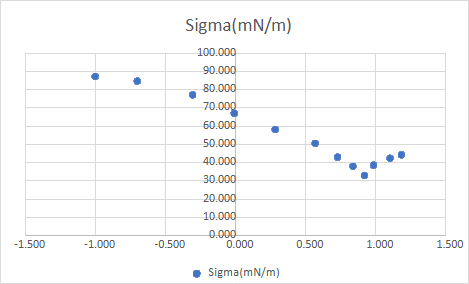
\includegraphics[width=0.8\textwidth]{bilder/diagramm1.png}
            \end{figure}

        \subsection{Diskussion}
            
            Zuerst zu den Abweichungen zum Literaturwert. Das Pulver zum anmixen der SDS-Lösung war schon älter und damit auch nichtmehr so rein wie es sein müsste um gute Ergebnisse zu erzielen. Da wir aus dem Skript wissen das Verunreinigungen die Oberflächenspannung erhöhen. Weiter war komplett sauberes Arbeiten nicht möglich und auch die Temperatur entsprach nicht der in der Literatur. Was man aber analog zu Literatur erkennt ist, dass die Kurve erst annährend wie eine Gerade fällt, also die Oberflächenspannung immer abnimmt. Bis der tiefste Punkt, die ideale Konzentration erreicht ist. Danach steigt die Oberflächenspannung wieder an. Das die Werte wieder ansteigen liegt daran, dass die Lösung komplett gesättigt ist und die Oberflächenspannung durch die Unreinheiten wieder ansteigt.

    \section{Versuch 3 - Oberflächenspannung von Wasser und SDS-Lösung mit der Kapillarmethode}

        \subsection{Aufbau}

            \begin{figure}[H]
                \centering
                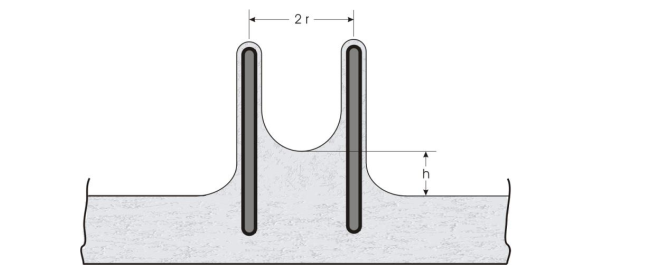
\includegraphics[width=0.8\textwidth]{bilder/Kapillarmethode.png}
                \caption{Versuchsaufbau Versuch 3 \ref{an:Anleitung}}
                \label{fig:Versuch3_Aufbau}
            \end{figure}

            \textcolor{red}{TODO: Aufbau beschreiben}

        \subsection{Auswertung}
            
            \begin{table}[H]
                \centering
                \caption{Messwerte Versuch 3}
                \label{tab:Versuch3_Ergebnisse}
                \vspace{0.8em}
                \begin{tabular}{|l|l|l|l|l|l|}
                    \hline
                    Durchmesser $\mathrm{[mm]}$ &  $\frac{1}{r}\mathrm{\left[\frac{1}{mm}\right]}$ &
                    $h_{\text{Demin, F}} \mathrm{[mm]}$ &
                    $h_{\text{SDS, F}} \mathrm{[mm]}$ &
                    $h_{\text{Demin, K}} \mathrm{[mm]}$ &
                    $h_{\text{SDS, K}} \mathrm{[mm]}$\\
                    \hline \hline
                    $0.83$ & $2.41$ & $32.9$ & $25.0$ & $ 37.099$ & $23.085$\\
                    \hline
                    $1.20$ & $1.67$ & $23.2$ & $16.0$ & $ 24.743$ & $16.928$\\
                    \hline
                    $1.65$ & $1.21$ & $16.3$ & $10.5$ & $ 17.708$ & $10.190$\\
                    \hline
                    $3.10$ & $0.65$ & $7.3$ & $5.0$ & $9.365$ & $5.176$\\
                    \hline
                    $5.00$ & $0.40$ & $3.2$ & $3.5$ & $4.597$ & $3.138$\\
                    \hline
                \end{tabular}
            \end{table}

            Die Werte $h_{\text{Demin, F}} \mathrm{[mm]}$ und $h_{\text{SDS, F}} \mathrm{[mm]}$ beschreiben die Höhe der Wassersäule, gemessen mit dem Fernrohr. Dabei wurde die Differenz des Tiefsten und des Höchsten Punktes gemessen. Die anderen beiden Höhenwerte wurden mit der Kamera bestimmt. Der Durchmesser $d$ beschreibt den Innendurchmesser der Kapillaren.

            Die folgenden 4 Graphen stellen die Höhe der Wassersäule im Verhältnis zu $\frac{1}{r}$ dar. Dabei ist $r$ der Innenradius der Kapillare. Die Graphen sind in 2 Gruppen aufgeteilt. Die erste Gruppe beschreibt die Messwerte mit dem Fernrohr und die zweite Gruppe die Messwerte mit der Kamera.

            \begin{figure}[H]
                \centering
                \caption{Höhe der Wassersäule (Demin, F) im Verhältnis zu $\frac{1}{r}$}
                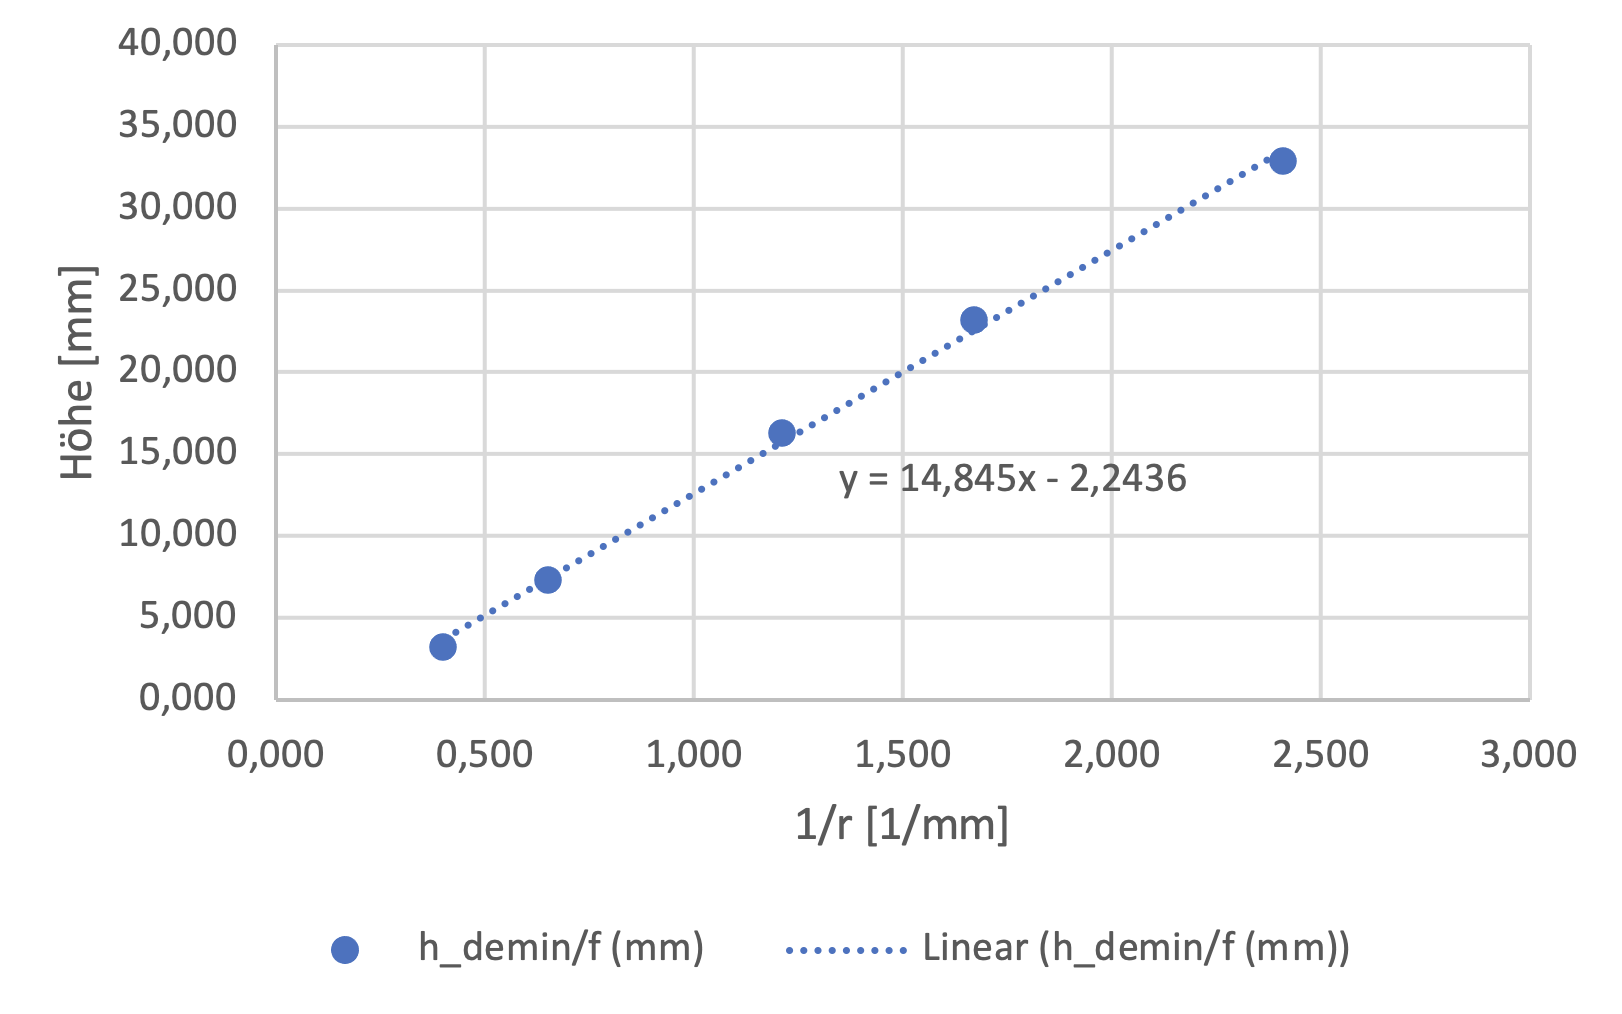
\includegraphics[width=0.8\textwidth]{bilder/graph_01.png}
                \label{fig:Versuch3_Graph1}
            \end{figure}

            \begin{figure}[H]
                \centering
                \caption{Höhe der Wassersäule (SDS, F) im Verhältnis zu $\frac{1}{r}$}
                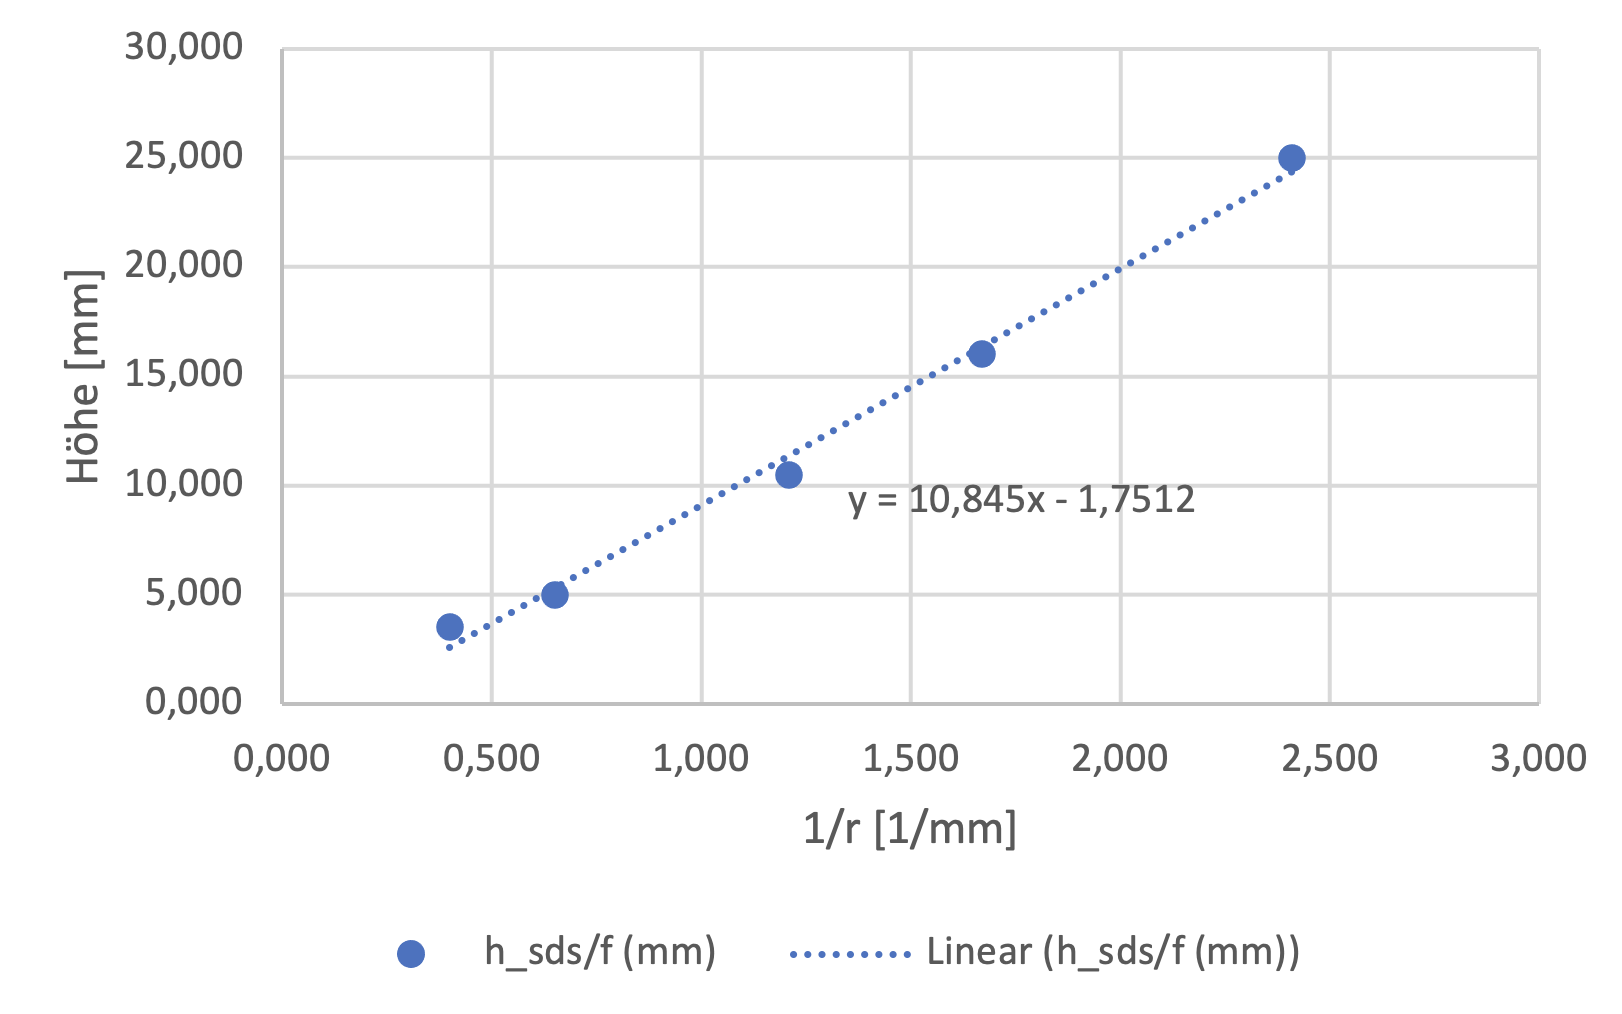
\includegraphics[width=0.8\textwidth]{bilder/graph_02.png}
                \label{fig:Versuch3_Graph2}
            \end{figure}

            \begin{figure}[H]
                \centering
                \caption{Höhe der Wassersäule (Demin, K) im Verhältnis zu $\frac{1}{r}$}
                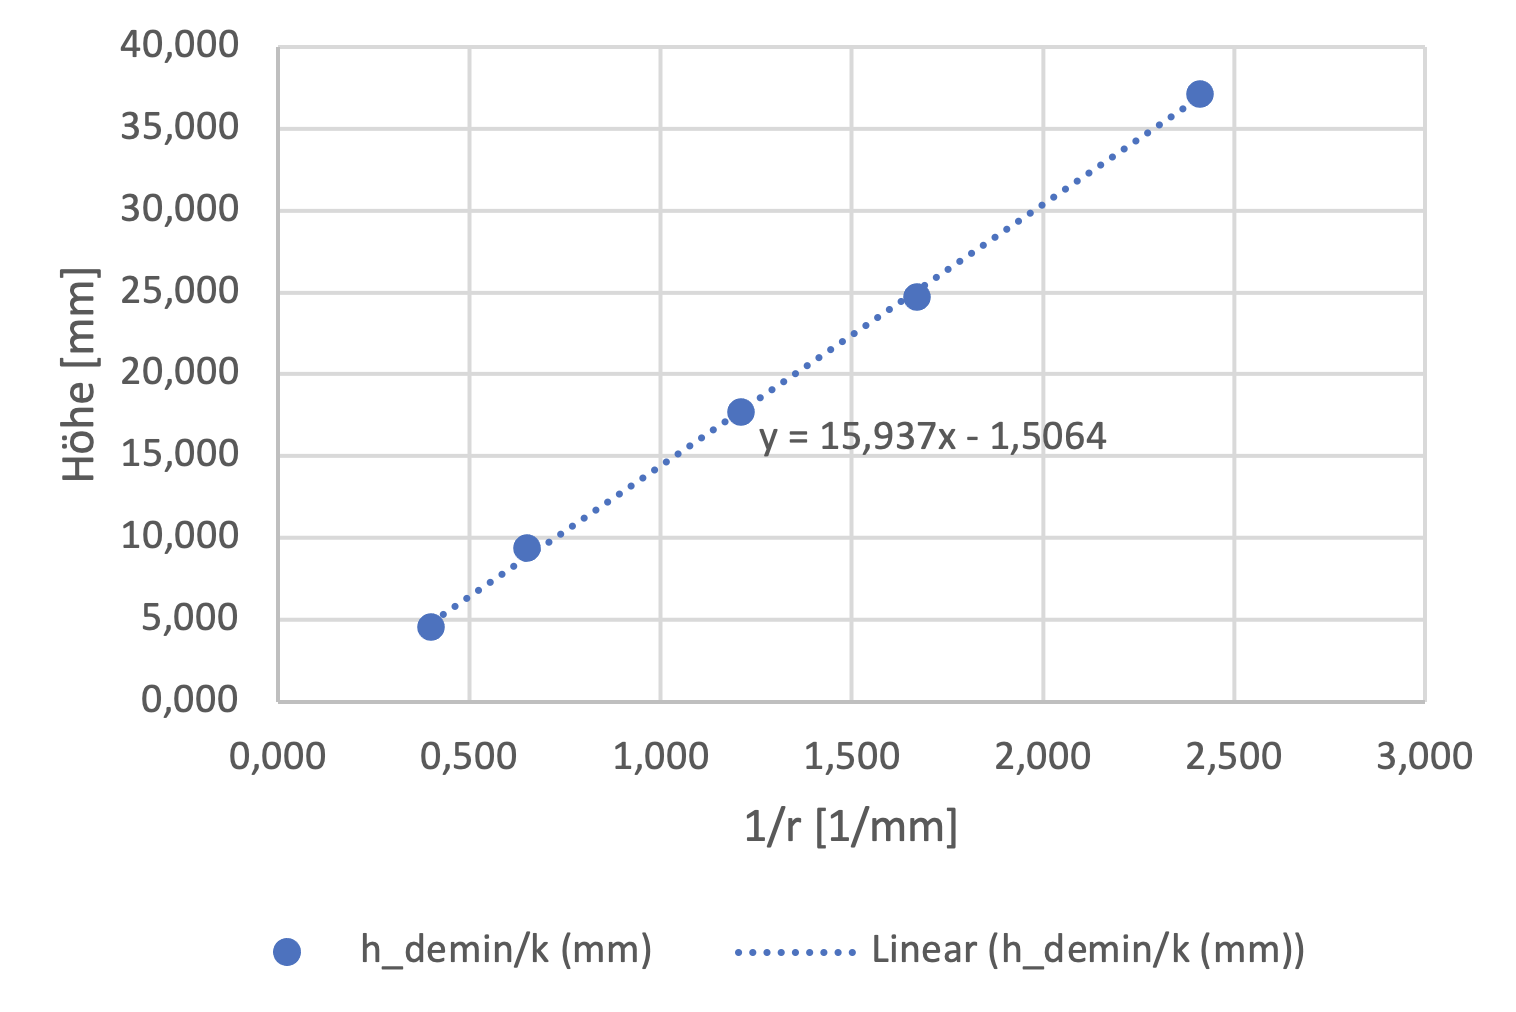
\includegraphics[width=0.8\textwidth]{bilder/graph_03.png}
                \label{fig:Versuch3_Graph3}
            \end{figure}

            \begin{figure}[H]
                \centering
                \caption{Höhe der Wassersäule (SDS, K) im Verhältnis zu $\frac{1}{r}$}
                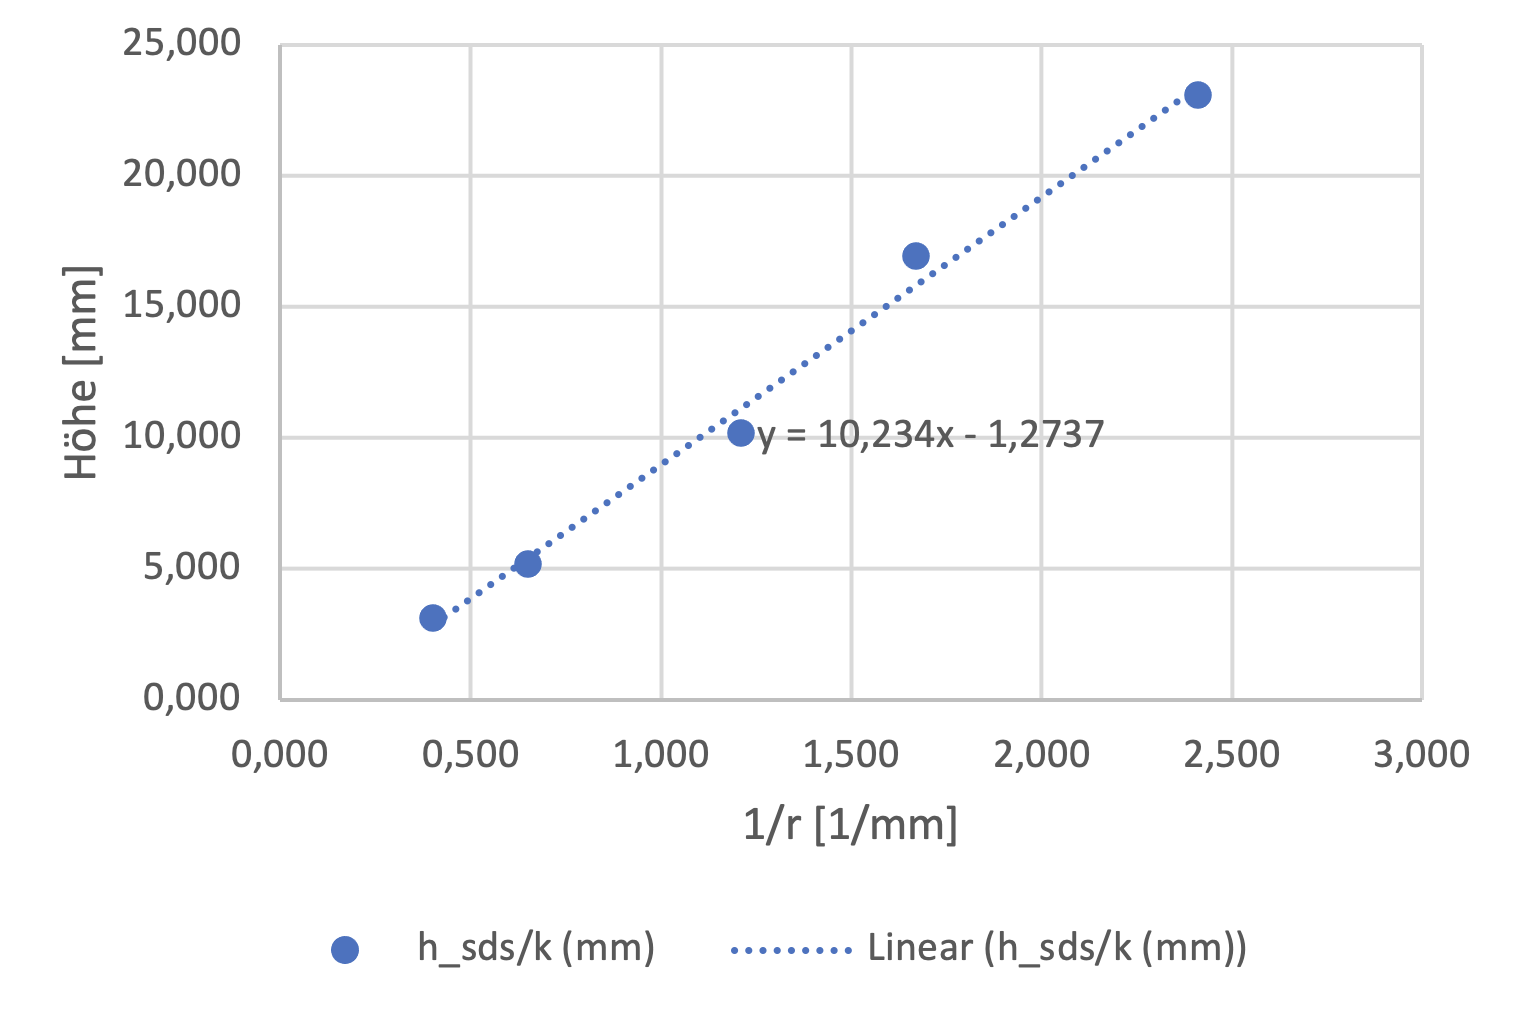
\includegraphics[width=0.8\textwidth]{bilder/graph_04.png}
                \label{fig:Versuch3_Graph4}
            \end{figure}

            Aus diesen Graphen lassen sich die Steigungen der Geraden ablesen. Anhand der Steigung und mit der folgenden Formel lässt sich nun wieder die Oberflächenspannung $\sigma$ berechnen.

            \begin{equation}
                \sigma = \frac{1}{2} \cdot \rho g m
                \label{eq:Oberflächenspannung_Kapillarmethode}
            \end{equation}

            \textcolor{red}{TODO: Formel checken}

            Die Dichte des Wasser beträgt $\rho = 0.998 \frac{\mathrm{g}}{\mathrm{cm^3}}$ und $g = 9.81 \frac{\mathrm{m}}{\mathrm{s^2}}$.

            Die Ergebnisse finden sich in folgender Tabelle:

            \begin{table}[H]
                \centering
                \caption{Ergebnisse Versuch 3}
                \label{tab:Versuch3_Ergebnisse}
                \vspace{0.8em}
                \begin{tabular}{|l|l|l|}
                    \hline
                    Flüssigkeit \& Methode & Steigung Graph & Oberflächenspannung $\sigma \mathrm{\left[\frac{mN}{m}\right]}$\\
                    \hline \hline
                    Demineralisiertes Wasser (Fernrohr) & $14.845$ & $72.596$\\
                    \hline
                    SDS (Fernrohr) & $10.845$ & $53.035$\\
                    \hline
                    Demineralisiertes Wasser (Kamera) & $15.937$ & $77.936$\\
                    \hline
                    SDS (Kamera) & $10.234$ & $50.047$\\
                    \hline
                \end{tabular}
            \end{table}

            \textcolor{red}{TODO: Formel für Sigma}

        \subsection{Diskussion}

            \textcolor{red}{TODO: Diskussion}